\section{Results}

\subsection{Operating principle}
Zapit is best thought of as a software-based solution for galvo-based photo-stimulation. 
Whilst we provide hardware designs (see below), there is no fixed design that is required to work with the software.
A variety of hardware designs can work and Zapit is flexible enough to take this into account. 

Here we implemented a hardware design similar to that used in \citet{Pinto2022MultipleCortex}.
A 470~nm laser is fed into an XY galvo scan block then is pointed down to the animal via a dichroic fold mirror.
A 100~mm achromatic lens focuses the beam onto the sample.
This lens doubles as an objective: imaging the sample and any excited green fluorescence onto a camera via a 50~mm tube lens (Fig.~\ref{fig:operating_principle_01}A).
The galvo waveforms are shaped to make them near inaudible, but nonetheless we designed a sealed enclosure for the scanners (Fig.~\ref{fig:operating_principle_01}B).

The Zapit software comprises of a user-friendly GUI for performing the two critical alignment steps. 
\textbf{1.} Aligning the scanners with the camera, enabling the beam to point accurately to any desired location in the image. 
\textbf{2.} Mapping stereotaxic coordinates onto the exposed skull.  
Calibration takes about a minute and, once calibrated, the system will place the beam in any desired location defined by stereotaxic coordinates. 

Once calibrated, a simple API allows the user to integrate stimulation into an experimental paradigm. 
The system currently supports stimulation of either one or two points in a given trial (extending it to more points is planned for the near future). 
In any given trial the laser spot either sits on one point and flashes on and off at 40~Hz or it goes back and forth between two spots in a 50/50 duty cycle illuminating each at 40~Hz. 
The location(s) of the beam in each stimulus condition is defined in stereotaxic coordinates.
There is a ramp down in intensity at trial end to avoid rebound effects. 
An optional blue LED masking light runs in synchrony with the laser.

\begin{figure}[h]
\centering
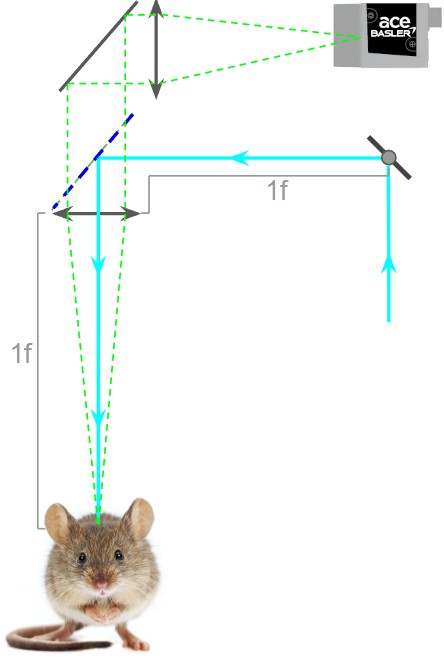
\includegraphics[width=0.325\textwidth]{Figures/Operating_Principles/Zapit_operating_principle_light_path.jpg}
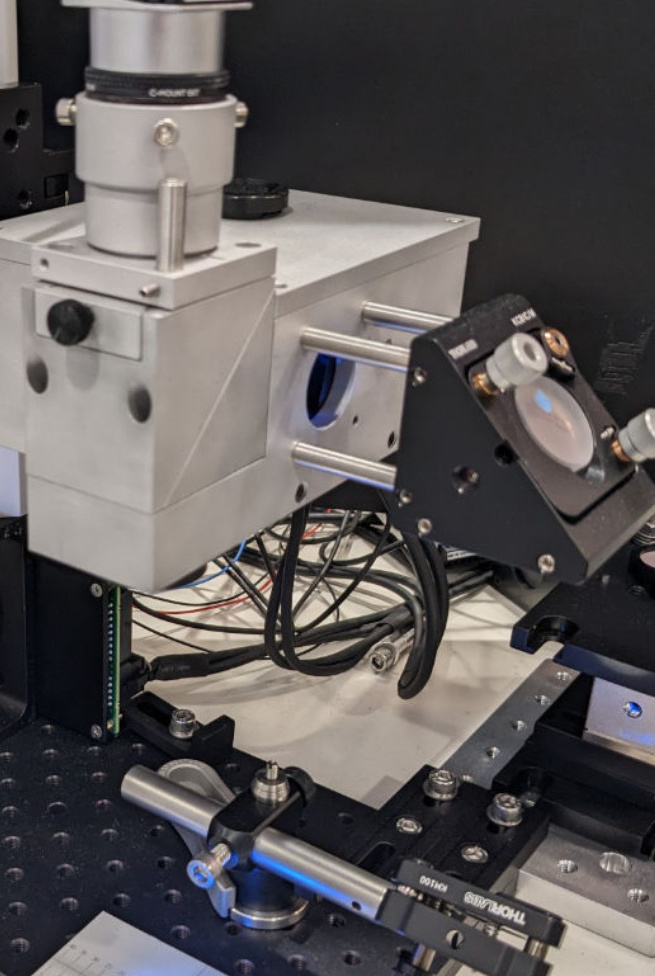
\includegraphics[width=0.325\textwidth]{Figures/Operating_Principles/Zapit_example_system_photo.jpg}
\caption{\textbf{A}. Optical path schematic.
A laser beam (blue) is directed using a pair of scan mirrors then focused through a lens and onto the skull surface via  dichroic mirror. 
The lens is located 1f from the scanners so that it behaves telecentrically. 
The dichroic allows the sample to be imaged on a camera via a tube lens
The beam location on the skull surface is visible due to autofluorescence. 
\textbf{B}. A photographed of an assembled system in a custom-built aluminum enclosure.}
\label{fig:operating_principle_01}
\end{figure}


\subsection{Hardware Design}

Details on the enclosure. 
Details on the Thorlabs CAD model.
Theoretical laser spot size is xx~$\mu m$.
PSF: theory. predicted. 

\begin{figure}[h]
\centering
\includegraphics[width=0.6\textwidth]{example-image}
\caption{A. Optical path schematic. B. Maybe a Zemax diagram. C. Photo of the system. D. Photo of the system.}
\label{fig:hardware01}
\end{figure}

\subsection{Software Design}
Explain how the software achieves the above.
A GUI allows specifying of points in stereotaxic coords and hence creation of settings files with respect to the Allen Atlas (Fig.~\ref{fig:software01}). 
Describe where this came from: the cortex lab and is that used by IBL.
Another GUI is used to calibrate the scanners such that they are able to point to locations in the image defined by the user. 
A second step defines the position of the skull in the FoV and hence previously specified stereotaxic coords can be overlaid onto the sample. 
The GUI has tools to allow visual confirmation of the scan and sample calibration steps (Fig.~\ref{fig:software02}).  

\begin{figure}[h]
\centering
\includegraphics[width=0.6\textwidth]{example-image}
\caption{Screenshot of stim config editor}
\label{fig:software01}
\end{figure}


\begin{figure}[h]
\centering
\includegraphics[width=0.6\textwidth]{example-image}
\caption{A. Screenshot of scanner calibration process. 
B. Screenshot of sample calibration process.}
\label{fig:software02}
\end{figure}


\subsection{Calibration}

The user initiates an automatic calibration procedure that maps the galvo control signals to pixel locations in the image. 
A simple two-click interface allows the user to map stereotaxic coordinates onto the image space. 

\subsection{Running Experiments}
Once the system is calibrated and a stimulus configuration file is loaded, it becomes possible to run an experiment.
There is an API available in MATLAB. 
The \texttt{sendSamples} command defines which stimulus will be presented next. 
By default the system queues the stimulus and waits for a TTL trigger before presenting it.
The \texttt{stopOptostim} command stops the stimulus whilst ramping down laser power over a user-defined time period.
If an `experiment directory' is defined in Zapit, \texttt{sendSamples} will write there a log file listing each stimulus presentation.
Control trials are possible where the galvos move and the masking light is on but the laser is off.

\lstinputlisting[language=MATLAB]{code_snippets/basic_api_example.m}

\subsection{Control via Python}
The `zapit-Python-Bridge' (installed via PyPI) provides access to the MATLAB API via shared memory. 
The user must start Zapit in MATLAB and conducted the scanner and sample calibration steps. 
All subsequent operations can be done via Python with commands that resemble those used in MATLAB.
For example:

\lstinputlisting[language=Python]{code_snippets/one_stim_example.py}

Zapit must remain running in MATLAB throughout. 


\subsection{Other languages}
Users wishing to use a different programming language must re-implement the \texttt{sendSamples} and \texttt{stopOptoStim} commands. 
This is straightforward and We provide minimal examples in the main Zapit repository to assist with this. 



\subsection{Validation}
\subsubsection{Scanner calibration accuracy}
Accuracy with which beam points to target in microns.
How the hell do we measure this? Using the camera? 
But then how accurate is our estimate of where the beam actually went? 
I guess we can show many points indicating where the beam went over many trials. 
That will show up bias.
But spread around the target location could be due to pointing errors or it could be due to errors in locating the beam. 
We can correlate with the galvo feedback waveforms and so know the error.
(Fig.~\ref{fig:validation01}A).

\subsubsection{Repeatability and Stability}
Have it run, say, 1000 trials of two locations quite far apart and record the command waveforms, galvo feedback, and beam intensity (Fig.~\ref{fig:validation01}B). 
Overlay these and show consistency over long periods of time and many trials. 
Feedback signals show us that the beam has arrived at the target location before being switched back on. 

\begin{figure}[h]
\centering
\includegraphics[width=0.6\textwidth]{example-image}
\caption{A. Scanner accuarcy
B. Repeatability and stability.}
\label{fig:validation01}
\end{figure}


\subsubsection{Suitability}
Measure laser power over the FOV and confirm it is the same everywhere (IT IS).
